\documentclass[a4paper,11pt,openany]{article}
\usepackage[noconfigs,french]{babel}
\usepackage[utf8]{inputenc}
\usepackage[left=2.5cm,right=2.5cm,top=1.5cm,bottom=1.5cm]{geometry}
\usepackage{amsmath}
\usepackage{amssymb}
\usepackage{float}
\usepackage{appendix} 
\usepackage{graphicx}
\usepackage{hyperref}
\usepackage{listings}  
\usepackage{mathtools}
%\usepackage{algorithm}
%\usepackage{algorithmic}
\usepackage[]{algorithm2e}
\usepackage{listings}
\usepackage{xcolor}
\lstset { %
    language=C++,
    backgroundcolor=\color{black!5}, % set backgroundcolor
    basicstyle=\footnotesize,% basic font setting
}



\title{Regroupement en diamants : structure de données compacte pour maillages tetrahédriques}
\author{Gabriel Beauplet, Luca Castelli Aleardi, Olivier Devilliers}
\date{%
    Stage de M2 MPRI\\%
    \today
}

\begin{document}
\maketitle

\section{Abstract}
\noindent
De nombreuses structures de données compactes ont été développées pour les triangulations 2D mais très peu pour les tétraèdrisations 3D. Nous introduisons dans ce rapport, une nouvelle structure de donneés compacte pour les tétraèdrisations. Nous nous concentrons seulement sur les informations de connectivité plutôt que sur les informations géométriques (les coordonnées des sommets). L'idée principale est de regrouper les tétraèdres en diamants de telle manière à économiser les références d'adjacence entre deux tétraèdres du même diamant. Nous définissons un diamant comme un ensemble de tétraèdres formant un cycle autour d'une arête. Notre structure de données permet de représenter la connectivité d'un maillage en utilisant en moyenne 2.4 références par tétraèdre tout en permettant l'exécution de requêtes simples. Nous présentons des résultats pratiques de notre structure de donneés ainsi que des résultats plus théoriques.
\section{Introduction}
\noindent
Un maillage représente un domaine géometrique en le discretisant en formes simples. Les maillages permettent de représenter des objets géométriques en 1, 2 ou 3D à des fins scientifiques ou industrielles par exemple. En 2D, les maillages representent des surfaces et sont constitués de polygones (triangles, carrés...) reliés deux à deux par une arête. En 3D, les maillages représentent des volumes à l'aide de polyèdres (tétraèdres, pyramides...) partageant une face commune. Les maillages sont très utilisés pour la visualisation de volume, calculs de solutions pour des équations aux dérivées partielles... Cependant, les maillages sont des structures complexes qui peuvent devenir très volumineuses et dont on essaye de réduire la taille.\\
La compression de données est omniprésente en informatique, avec des formats compressés génériques comme \textit{gzip} mais aussi dédiés comme \textit{mp3} pour les fichiers audios. Ce besoin de compresser les données est grandissant car de plus en plus de fichiers sont stockés à distance sur des serveurs et la moindre économie de stockage a d'importantes répercussions. Néanmoins, sous certains formats compressés, les données originales deviennent inutilisables (ex : \textit{rar}). Cela pose problème quand l'on souhaite accéder aux données  sans passer par l'étape de décompression.\\
Une structure de données est une manière d'organiser les données pour faciliter leur traitement. Les listes, arbres et graphes sont des exemples de structures de données. Leur but n'est pas de limiter l'usage mémoire mais seulement de faciliter l'utilisation des données. Ainsi, pour certains formats volumineux, des structures de données compactes ont été inventées. Ce sont des structures de données compressées, des structures de données dont l'utilisation de la mémoire est limitée.\\
Si l'on revient aux maillages, les algorithmes de compression limitent au maximum l'usage mémoire du maillage et il devient inutilisable sous forme compressé tandis que la structure de données pré-traite le maillage en réduisant l'usage mémoire mais celui-ci reste utilisable. Les maillages en deux dimensions sont majoritairement utilisés car ils sont plus léger, et permettent de représenter implicitement des volumes (la frontière). Par conséquent, de nombreuses structures de données compactes ont été créees afin de faciliter leur utilisation. Les maillages 3D étant beaucoup moins utilisés pour l'instant, peu de structure de données compactes leur sont dévolues. Néanmoins, leur utilisation croissante incite à procéder de même. La suite de ce rapport sera principalement consacrée aux structures de données compactes pour maillages 3D tétraèdriques.\\\\
De manière générale, un structure de données pour maillage stocke trois types d'informations :
\begin{itemize}
\item La géometrie, c'est à dire les positions des sommets
\item La connectivité, les relations d'adjacence entre les tétraèdres
\item Des attributs (par sommet, par arête, par face, par tétraèdre)
\end{itemize}
La structure de données doit supporter des requêtes simples :
\begin{itemize}
\item Quels sont les sommets de la ième face ?
\item Quel est le degré du ième sommet ?
\item Quelles sont les tétraèdres adjacents au ième tétraèdre ?
\item ...
\end{itemize}
Par ailleurs, suivant l'utilisation ciblée, la structure de données devra être en mesure de satisfaire des opérations de modification :
\begin{itemize}
\item Ajouter/Enlever un sommet
\item Ajouter/Enlever/Séparer un tetra\\
\end{itemize}
%Finalement, le fonctionnement de la structure de donnée doit être simple pour permettre sa ré-implémentation.\\
On évalue une telle structure de données en analysant le temps nécessaire à sa construction, à l'exécution d'une requête, à une opération de modification et surtout en observant la quantité de stockage nécessaire pour l'utiliser.\\\\
\textbf{Contributions}. Dans ce rapport, nous présentons une structure de données permettant de représenter la connectivité d'un maillage tetrahedrique en utilisant en moyenne 2.4 références par tétraèdre. Notre structure s'appelle \textit{Tétraèdres en diamant}. Elle permet par ailleurs l'accès au ième sommet, au ième tétrahèdre et à l'étoile d'un sommet en temps constant. Son implémentation est simple et l'utilisation d'un tableau d'entiers afin de représenter les références permet une interopérabilité entre les languages de programmation.\\
Nous allons d'abord définir les principaux termes utilisés et rapeller les algorithmes de compression et structures de données déjà développés en deux et trois dimensions. Puis nous présenterons le fonctionnement, les avantages et inconvénients de notre structure de données. Par ailleurs, nous comparerons notre structure de données avec d'autres structures en terme de stockage mémoire ou de coût de calcul.

\subsection{Définitions}
\noindent
\textbf{Simplexe}. Un simplex $\sigma^p$ de dimension $p$ est l'enveloppe convexe de $p+1$ points $\{v_0,v_1,...v_p\}$, où $v_i\, \in R^n$ et les vecteurs $v_1-v_0,v_2-v_0...$ sont linéairement indépendants. Les simplexes de dimensions 0, 1, 2 et 3 sont respectivement les sommets, arêtes, triangles et tétraèdres.\\\\
\textbf{Complexe simplicial}. Un complexe simplicial est un ensemble K de simplexes d'un espace affine tel que toutes les faces de chaque simplexe de K appartiennent aussi à K et si deux simplexes $\sigma$ et $\tau$ de K sont adjacents alors $\sigma \cap \tau \neq \emptyset$.\\\\
%Les points $v_0,v_1,...v_p$ sont appelés les sommets de $\sigma$. 
%Une face est l'enveloppe convexe d'une partie des sommets (pas tout). Si un simplex $\sigma$ est la face d'un simplexe $\tau$, alors $\tau$ est dit incident et $\tau$ limite $\sigma$. La frontière d'un p-simplexe $\sigma$ $\partial \sigma$ est la collection de toutes ses faces.\\\\
%\textbf{Etoile}. L'étoile ouverte d'un simplexe $\sigma \in K$ noté étoile($\sigma$,$K$) est l'union de tous les simplexes de l'étoile avec ses faces.\\\\
\textbf{Variété}. Une variété topologique (manifold en anglais) M de dimension n est un espace topologique connexe séparé localement homéomorphe à un ouvert de $\mathbb{R}^n$. C'est à dire que chaque point de M admet un voisinnage homéomorphe à un ouvert de $\mathbb{R}^n$.\\\\
\textbf{Variété à bord}. Une variété à bord est un sous-espace topologique dont les points admettent un voisinage homéomorphe à $\mathbb{R}^n$ (les points intérieurs) ou un voisinage homéomorphe à $\mathbb{R}^{n-1}  x \mathbb{R}^+$ (les points bordants). L'ensemble des points bordants constitue le bord de la variété.\\\\
\textbf{Frontière}. Les (k-1)-simplexes d'une k-variété $M$ qui sont incidents à seulement un k-simplexe sont les simplexes frontières. L'ensemble des simplexes frontières est dénoté $\partial M$.\\\\
%Une k-variété est orientable s'il est possible de choisir une orientation cohérente pour tout ses simplexes. Une orientation est cohérente si deux k-faces adjacentes induisent deux orientations opposées sur leur (k-1)-face.
%Un complexe simplicial  $M$ est une k-variété si l'étoile ouverte d'un sommet dans $M$ est homeomorphique à $R^k$ ou à $R^{k-1}XR_+$. En particulier, si $M$ est une variété alors tout (k-1)-simplex dans $M$ est la frontière de un ou deux k-simplexe.\\
\textbf{Maillage}. Un maillage est un complexe simplicial representant un objet géométrique. Il à la même dimension que l'objet qu'il représente. Ainsi, pour tout objet en 1, 2 ou 3D, les maillages respectifs seront en dimensions 1, 2 ou 3. Dans un maillage de dimension d, les simplexes de dimensions (d-1) sont appelées des facettes. Ainsi, les facettes d'un tétraèdre sont ses faces, les facettes d'une face sont ses arêtes et les facettes d'une arête sont ses sommets.\\\\
\textbf{Le degré}. Le degré d'un k-simplexe est le nombre de (k+1)-simplexes adjacents. Ainsi le degré d'un sommet est le nombre d'arêtes adjacentes et le degré d'une arête est le nombre de faces adjacentes.\\\\
\textbf{Etoile}. L'étoile d'un sommet est l'ensemble des k-simplexes adjacents à un sommet. C'est l'ensemble des triangles (resp. tétraèdres) adjacents à un sommet dans le cas surfacique (resp. volumique). Dans ce dernier cas, on appelle cela l'hypersphère.\\\\

%Nous traitons dans ce rapport de maillages tetrahedriques dans un espace Euclidien à 3 dimensions. Deux tetrahedres sont dit adjacents s'ils partagent une face. On dénote par V l'ensemble des sommets, E l'ensemble des arêtes, F l'ensemble des faces et T l'ensemble des tetrahedres du maillage.\\
%En utilisant l'équation d'Euler, on a la relation suivante : 
%\begin{equation}
%|V|-|E|+|F|-|T|=\chi
%\end{equation}

\subsection{Combinatoire}
\noindent
En mathématique et en optimisation combinatoire, la caracéristique d'Euler $\chi$ est un invariant topologique décrivant la forme d'un objet géométrique.
\begin{equation}
\chi = \sum_{i=0} (-1)^i \, |dim(H_i)| = 2-2g
\end{equation}
\begin{itemize}
\item $H_i$ est l'ensemble des faces de dimension $i$
\item $g$ est le genre (le nombre de trou de l'objet étudié)\\ 
\end{itemize}
Ainsi, pour un polytope de dimension 4, la formule d'Euler devient :\\
\begin{equation}
\chi = |V|-|E|+|F|-|T|
\end{equation}
\begin{itemize}
\item $V$ est l'ensemble des sommets
\item $E$ est l'ensemble des arêtes
\item $F$ est l'ensemble des faces (ie. polygone)
\item $T$ est l'ensemble des tétraèdres\\
\end{itemize}
Sachant que chaque face qui n'est pas sur les bords du volume est partagée par deux tétraèdres, alors :\\
\begin{equation}
|F|\simeq 2|T|
\end{equation}
Ainsi :
\begin{equation}
\chi \simeq |V|-|E|+|T|
\end{equation}
Il y a donc autant d'arêtes que de tétraèdres et sommets réunis.

\section{Etat de l'art}
\noindent
Les maillages sont la pluspart du temps stockés sous forme indexés. Dans un premiers temps, on énumère pour chaque sommet ses coordonnées géométriques. Puis pour chaque face (resp. tétraèdre), les indices de ses 3 (resp. 4) sommets. D'autres attributs peuvent être stockés (normales, couleurs...) mais nous n'en discuterons pas ici. Les formats indexés ne sont pas les formats les plus concis pour sauvegarder des maillages. En effet, la connectivité occupe une place très importante. Tandis que dans les maillages 2D, le degré moyen des sommets est de 6, il est de 22 dans les maillages tétraèdriques. Par conséquent, dans ce type de format, un sommet apparaitra dans 22 tetras différents.\\
%La compression de maillages peut être séparer en 3 catégories : simplification polyhedrale, compression de positions, compression des informations de connectivités.\\\\
%\textbf{La simplification polyhedrale} consiste à simplifier le maillages en réduisant le nombre de sommets et en modifiant leurs positions afin que le nouveaux maillages reste aussi proche que possible de l'ancien. Ce sont des compression de maillages avec perte et ne sont donc pas adaptés aux usages nécessitant le maillage exact.\\\\
%\textbf{Compression des positions}\\\\
%\textbf{Compression de la connectivite}. La compression des informations de connectivité permet de réduire la redondance d'informations d'adjacence entre les k-simplexe d'un k-objet.\\\\
%En effet, comme dit dans la première partie, la structure de données doit être capable de répondre à des requetes simples (ex: donner les tetras adjacents à un tetra). Sans compression, cela signifie que chaque tetra doit stocker 4 références vers ses 4 tetras voisins. De plus, si l'on veut connaître les sommets composants un tetra, il est nécessaire de sauvegarder 4 references vers les 4 sommets composant le tetra. Ainsi, nous avons 8 références par tetra. Par conséquent, dans un maillage contenant 10000 tetras et en utilisant des références sur 32 bits, nous utiliserions 10000*8*32=2mo de références.
%On distingue les algorithmes de compression de maillages des structure de données pour maillages. Les premiers tentent de limiter au maximum l'usage mémoire du maillage en compressant le maillage. Le maillage devient inutilisable sous forme compressé, il est nécessaire de le décompresser pour l'utiliser à nouveau. En revanche, la structure de données pré-traite le maillage mais le maillage reste utilisable sous forme compressé.\\
La mesure utilisée pour évaluer la qualité d'une compression est le nombre de bits par sommets (bits per vertex ou bpv). Tandis que la mesure utilisée pour évaluer la qualité d'une structure de données compacte est le nombre de références par triangle (resp. tétraèdre) rpt pour les maillages surfaciques (resp. volumiques).\\
On peut compresser un maillage en le simplifiant (supprimer des sommets...), en encodant la géométrie et/ou la connectivité du maillage. Nous ne nous intéresserons dans cette partie qu'à la compression de la connectivité puisque c'est la plus gourmande en mémoire. Par ailleurs, nous détaillerons d'abord le travail effectué en 2D puis en 3D. Bien que notre travail soit uniquement centré sur les maillages 3D, l'essentiel des travaux effectués jusqu'à présent est en 2D.
\subsection{Maillages 2D}
\subsubsection{Compression}
\noindent
\textbf{Bande de triangle}. Les bandes de triangles ("triangles strips") et les eventails de triangles ("triangle fans") sont des représentations utilisées pour transférer les maillages de la mémoire centrale du PC vers la mémoire du GPU. Une bande de triangle est une séquence de sommet où chaque nouveau sommet défini un triangle avec les deux précedent sommets. En ce qui concerne les bande de triangles, le but est de trouver de très longues bandes. Si les bande de triangles sont suffisament longue alors, cette representation permet de passer de 3N references aux sommets à N+2. L'algorithme de Deering utilise ces bandes de triangles et utilise entre 3.3 et 9.8 bpv \cite{triangle_strips}.\\\\
\textbf{Traversée de triangles}. La Cut border Machine \cite{cut_border_machine_2d} est un algorithme de Gumhold qui encode la conectivité en parcourant le graphe en largeur. L'algorithme étend la frontière défini par un triangle initial en travesant itérativement des triangles adjacents. Sept symboles sont utilisés pour préciser si la frontière a été étendu en insérant un nouveau sommets, si la frontière a été séparée ou si deux frontière se sont jointes. Le schéma peut compresser des variétés avec 4 bpv. En revanche, ce résultat est seulement valide pour des maillages réguliers. En effet, quand une jointure est effectuée, un décallage doit etre fait pour désigner les sommets concernés. Par conséquent, il n'y a pas de borne supérieure garantie pour la compression avec cet algorithme.\\
L'algorithme EdgeBreaker de Rossignac \cite{edgebreaker} traverse lui aussi le graphe d'un triangle adjacent à un autre et enregistre la connectivité d'un maillage en produisant les sympboles C,L,R,E,S. Cependant, il garantit un cout de 4bpv.\\\\
\begin{figure}[H]
\begin{center}
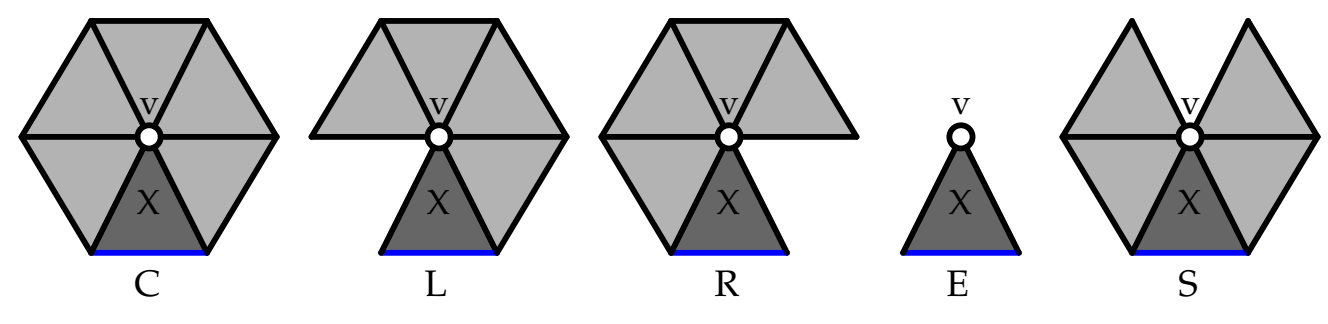
\includegraphics[scale=0.2]{Images/edgebreaker}
\caption{Les cinq configurations dans l'algorithme Edgebreaker. v est le sommet central de la configuration et X est le triangle cible}
\label{fig:edgebreaker}
\end{center}
\end{figure}
\noindent
\textbf{Codage de la Valence}. Une manière de décrire la connectivités de sommets est à travers leurs valence. Le premier travail sur la valence des sommets est le travail de Touma et Gotsman \cite{valence_encoding}. Le principe est de considérer la frontière d'un triangle initial et de l'étendre en ajoutant itérativement de nouveaux sommets. La connectivité est encodée en utilisant la valence des nouveaux sommets (concentrée autour de 6). Ainsi, La liste de valence des sommets peut être efficacement compressée par un encodeur d'entropie (2.3 bpv). C'est toujours aujourd'hui l'une des méthodes les plus efficace.
\subsubsection{Structure de données compacte}
\noindent
Plusieurs structures de données permettent une utilisation très facile des maillages et se focalisent sur l'utilisation des arêtes du graphe. C'est le cas d'Half-Edge, Winged-Edge et Quad-Edge qui stockent $19n$ références (soit 9.5 rpt). Elles permettent facilement de naviguer dans le maillage et opèrent des requêtes d'adjacence en temps constant. Cependant, elles occupent trop de place pour être considérées comme compactes.\\
La Corner Table (CT) est à la base de plusieurs structures de données. Elle utilise deux listes V et O de $3|F|$ entiers chacune. La table V stocke les incidence triangle/sommet tel que les 3 sommets bordant un triangle t sont consécutifs (V[3t],V[3t+1],V[3t+2]) et sont listés dans un ordre consistent avec le maillage. Ainsi, V[c] représente un coin c associé avec une face f et un sommet. La table O stocke la référence entière du coin oposé. Le coin opposé o(c) au coin c est un coin dans un triangle adjacent qui partage la même arête opposée.
\begin{figure}[H]
\begin{center}
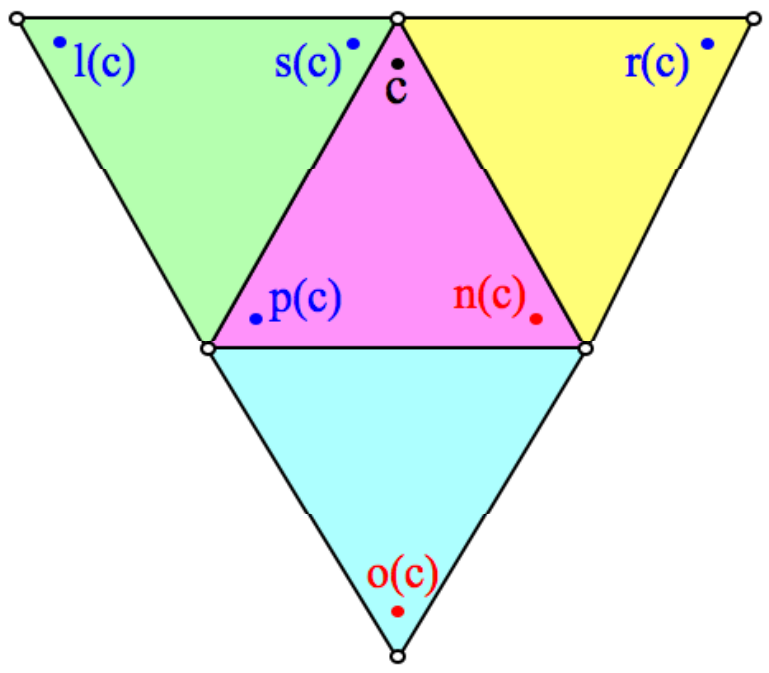
\includegraphics[scale=0.2]{Images/corner_table}
\caption{Les opérateurs utilisant les coins pour un maillage triangulaire}
\label{fig:corner_table}
\end{center}
\end{figure}
\noindent
\textbf{VOT}. La structure de données VOT (Vertex Opposite Table) est la première structure de données à utiliser cette "Corner Table". Elle permet une répresentation simple et efficace des maillages avec 6 références par triangle (3 références pour les sommets dans la table V et 3 référence pour les coins dans la table O).\\
\textbf{SOT}. SOT, développée par Rossignac \cite{SOT} est une amélioration de VOT où la table O est réordonnée et la table V supprimée. Néanmoins, l'accès au coin d'un sommet et à l'étoile d'un sommet sont toujours en temps constant. Cette dernière structure de données utilise 3 rpt en moyenne.

\footnotesize
\begin{tabular}{|c | c | c | c | c|}
\hline
Structure de données & Taille mémoire & Temps de navigation & Accès au sommet & Dynamique\\
\hline
Basées sur les arêtes\\(Half-edge, Quad-edge, Winged-edge) & 18n+n & O(1) & O(1) & oui\\
Basées sur les triangles & 13n & O(1) & O(1) & oui\\		
Corner table & 13n & O(1) & O(1) & oui\\
\hline
2D catalog & 7.67n & O(1) & O(1) & oui\\
\hline
Star vertices & 7n & O(d) & O(1) & non\\		
SOT & 6n & O(1) & O(d) & non\\
SQUAD & $(4+\epsilon)$n & O(1) & O(d) & non\\
LR & $(2+\delta)$n & O(1) & O(d) & non\\
\hline  
\end{tabular}

\normalsize
%\subsubsection{Enumération de triangulations planaires}
%La connectivité d'un maillage peut etre vu comme un graphe. Pour les maillages surfaciques, les sommets sont des noeuds connectés via les arêtes du graphes pour former des faces.
%%Cette analogie entre maillage et graphe explique pourquoi certains résultats très connu de la théorie des graphes peuvent etre appliqués pour la compression de la connectivité des maillages.
%Tutte a d'abord proposé une formule pour énumérer les triangulations planaires. Cette première énumeration permet de calculer ce que l'on appelle l'entropie de Tutte. Cette entropie vaut environ 3.25 bpv (bits per vertex). C'est une borne supérieure pour l'entropie de la connectivité de n'importe quel maillage surfacique.
\subsection{Maillages 3D}
\subsubsection{Compression}
\noindent
\textbf{Grow\&Fold}. L'algorithme Grow\&Fold \cite{grow_and_fold} combine les idées de l'algorithme Topological Surgery \cite{topological_surgery} de Taubin et EdgeBreaker \cite{edgebreaker} de Rossignac. Il construit un arbre couvrant de tétraèdre et un folding string. L'arbre couvrant début à une face arbitraire et grandit en ajoutant des tétraèdres aux faces externes de l'actuel arbre couvrant. Pour chaque ajout de tétraèdre, 3 bits encodes si d'autres tétraèdres seront attchés aux 3 faces extérieures de ce tétraèdre. Le folding string contient pour chaque triangle externe de l'arbre couvrant un code sur 2 bits permettant de retrouver les relations d'incidences absentes de l'arbre couvrant. L'abre couvrant contient $|T|$ tétraèdres et il y a $2|T|$ faces externes. Par conséquent, l'usage mémoire est de 7 bpt.\\
\textbf{Cut Border Machine}. La Cut Border Machine pour les maillages volumiques \cite{cut_border_machine_2d} est directement inspirée de celle pour les maillages surfaciques de Gumhold \cite{cut_border_machine_3d}. L'algorithme étend la frontière défini par une face initiale en traversant des tétraèdres adjacents. Dix symboles sont utilisés pour décrire l'entourage de la frontière lors de l'ajout d'un nouveau sommet pour la construction d'un tétraèdre. Leur algorithme permet de compresser les maillages tétraèdriques en utilisant 2.4 bpt et s'adapte aux non-variétés.
 
\subsubsection{Structure de données compacte}
\noindent
\textbf{VOT}. La Corner Table a été adapté par Rossignac aux maillages tétraèdriques (VOT). Elle demande 8 rpt (4 pour les sommets et 4 pour les coins opposés). Un index dans ces listes identifie un coin particulier à un tétraèdre. Ainsi, les tables O et V ont toutes les deux $4|T|$ entrées. Les coins de chaque tetrahèdre sont consécutifs dans les deux listes (les quatres coins du ième tetra sont stockées aux entrées  4i+j, where j = 0,1,2,3) et sont listés dans un ordre consistent avec l'orientation du tétrahèdre (les sommets des coins j=1,2,3 apparaissent dans le sens inverse des aiguilles d'une montre depuis le sommet du coin 0).\\
\textbf{Bande de Triangles}. Weiler et al. \cite{triangle_strips_weiler} encode les tétrahèdres en bandes. L'inclusion d'une petite quantité d'informations d'adjacence leur permet d'acceder aux faces voisines en temps constant. Leur algorithme stocke en moyenne 5.1 rpt.\\
\textbf{SOT}. La dernière structure de données développée est SOT \cite{SOT} par Rossignac. Elle améliore sa première structure de données VOT en triant la table O et en supprimant la table V. La structure de données utilise 4 références et 9 bits par tétraèdre en moyenne et permet l'accès à l'étoile d'un sommet en temps constant.

\section{Diamond Compression}
\subsection{Le principe}
\noindent
Dans SQUAD, les auteurs traverse le graphe en prodondeur afin d'apareiller les triangles deux à deux avec l'un de leurs sommet partagé. Cela leur permet d'avoir 4 références par quad (i.e pair de triangle) et donc d'économiser une référence par triangle. Quant aux triangles non appareillés, ils sont déguisés comme des quads. D'autre part, tout comme SOT, ils utilisent l'ordre des quads tel que le ième quad soit associé au ième sommet. Dans un maillage 2D, il y a deux fois plus de triangles que de sommets. Par conséquent, le nombre de quads et le nombres de sommets devrait être assez proche.\\
Notre algorithme s'inspire fortement de SQUAD. Seulement, appareiller les tétraèdres deux à deux permet seulement d'économiser une référence par cube, c'est à dire de passer de 4 références par tétraèdre à 3.\\
L'idée ici est de regrouper les tetrahedres partageant une même arête. On appelle un tel regroupement un diamant. Il combine les idées de plusieurs papiers :
\begin{itemize}
\item Regroupement des tétraèdres comme SQUAD
\item Ancrer un sommet avec un diamant comme SOT
\item Ordonner les diamants tel que le ième sommet soit au sein du ième diamant comme SOT
\item Passage d'un tétraèdre à l'autre en utilisant les faces (et non les coins)
\end{itemize}
Un diamant est un ensemble de tétraèdres adjacents deux à deux, partageant une arête commune et formant un cycle (fig. \ref{fig:full_diamond2}). Dès lors que l'ensemble des tétraèdres n'est pas cyclique, la figure géométrique n'est plus un diamant (fig. \ref{fig:not_full_diamond}). 
\begin{figure}[H]
\centering
\begin{minipage}{.5\textwidth}
  \centering
  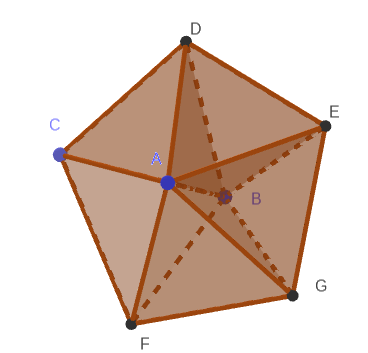
\includegraphics[scale=0.3]{Images/full_diamond}
  \caption{figure}{Exemple de diamant contenant 5 tétraèdres et dont l'arête centrale commune est AB}
  \label{fig:full_diamond2}
\end{minipage}%
\begin{minipage}{.5\textwidth}
  \centering
  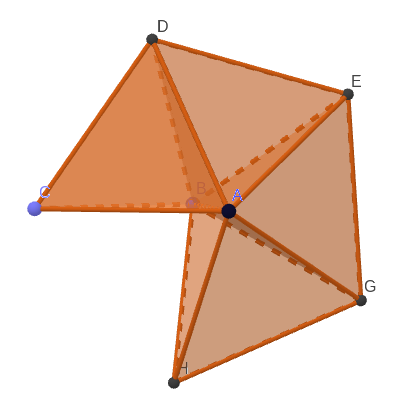
\includegraphics[scale=0.26]{Images/not_full_diamond}
  \caption{figure}{Exemple n'étant pas un diamant car les tétraèdres ne sont pas cycliques (bien que tous les tétraèdres partagent la même arête AB)}
  \label{fig:not_full_diamond}
\end{minipage}
\end{figure}
\noindent
Au sein d'un diamant, les tétraèdres sont ordonnés. Ainsi, on peut oublier les références de voisinage entre deux tétraèdres du même diamant. Par conséquent, pour les tétraèdres au sein d'un diamant, seules les références vers des tétraèdres extérieurs sont nécessaires. Un diamant D contenant $|D|$ tétraèdres aura $2|D|$ références. Si tous les tétraèdres sont réunis en diamants, notre structure consommerait 2 rpt.\\
Sur la figure \ref{fig:full_diamond2}, on peut ordonner les tétraèdres tel-que :
\begin{itemize}
\item Tétraèdre 0 : ABCD
\item Tétraèdre 1 : ABDE
\item Tétraèdre 2 : ABEG
\item Tétraèdre 3 : ABGF
\item Tétraèdre 4 : ABFC
\end{itemize}
Les faces ABD,ABE,ABG,ABF,ABC n'apparaitront pas dans notre structure car nous savons implicitement que pour passer d'un tétraèdre à l'autre dans ce diamant, nous utilisons une de ces faces.\\
\subsection{Evalution de notre structure de données}
\noindent
Il est évident que nous devons évaluer notre structure afin de comparer ses performances aux résultats pré-existants. Pour cela, nous avons choisi une dizaine de maillages avec des formes, des tailles, et des tétraèdrisations différentes. La pluspart des maillages ont été réalisés avec la bibliothèque CGAL \cite{CGAL}. Nous ne présentons les résultats de nos algorithmes que sur 6 de ces maillages.
\begin{figure}[H]
\centering
\begin{minipage}{.5\textwidth}
  \centering
  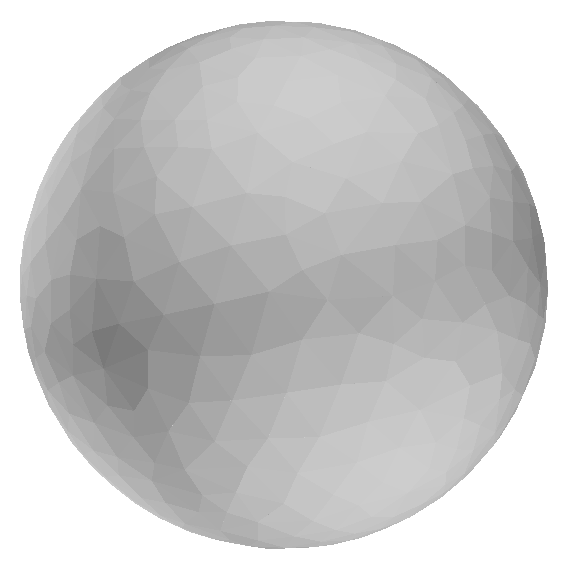
\includegraphics[scale=0.2]{Images/ball}
  \caption{figure}{Tétraèdrisation d'une boule}
  \label{fig:ball}
\end{minipage}%
\begin{minipage}{.5\textwidth}
  \centering
  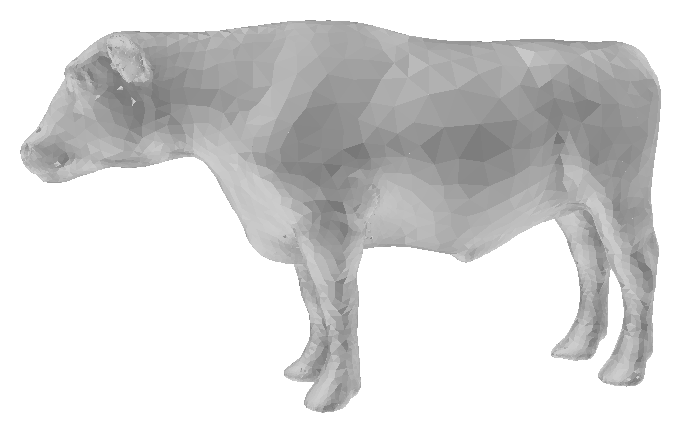
\includegraphics[scale=0.2]{Images/cow}
  \caption{figure}{Tétraèdrisation d'une vache}
  \label{fig:cow}
\end{minipage}
\end{figure}

\begin{figure}[H]
\centering
\begin{minipage}{.5\textwidth}
  \centering
  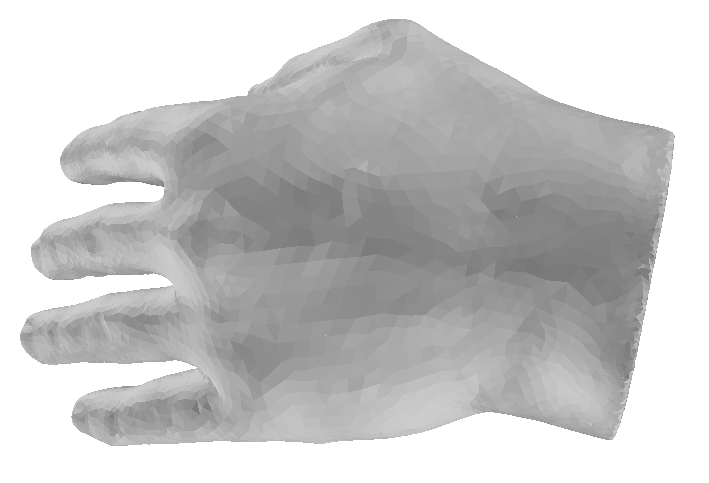
\includegraphics[scale=0.2]{Images/hand}
  \caption{figure}{Tétraèdrisation d'une main}
  \label{fig:hand}
\end{minipage}%
\begin{minipage}{.5\textwidth}
  \centering
  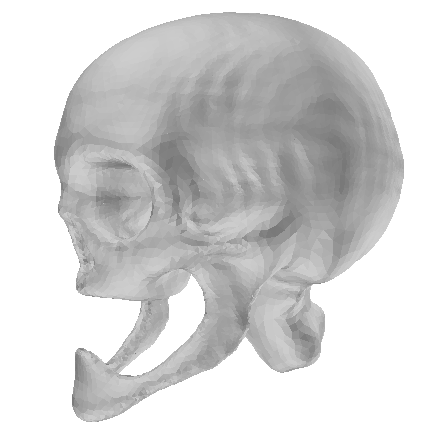
\includegraphics[scale=0.2]{Images/skull}
  \caption{figure}{Tétraèdrisation d'un crane}
  \label{fig:skull}
\end{minipage}
\end{figure}

\begin{table}[H]
\footnotesize
\begin{tabular}{|c | c | c | c | c| c | c |}
\hline
Nom de la & Nombre de & Nombre& Nombre de & Part de tétraèdres & Nombre de & Nombre d'arêtes\\
structure&sommets&d'arêtes &tétraèdres&sur les bords&tétraèdres par sommet & par sommet\\
\hline
Boule (B1) & 1056 & 5452 & 3583 & 0.45 & 13.52 & 10.32 \\
Boule (B2)& 15063 & 101343 & 83412 & 0.07 & 22.15 & 13.45\\
Boule (B3)& 378532 & 2647808 & 2243131 & 0.05 & 23.70 & 13.98 \\
Vache (V1)& 30808 & 182170 & 134707 & 0.24 & 17.48 & 11.82 \\
Main (M1)& 28796 & 169115 & 125127 & 0.24 & 17.38 & 11.74\\
Crane (C1)& 37813 & 217974 & 156135 & 0.30 & 16.51 & 11.52 \\ 
\hline  
\end{tabular}
\label{Tab:results_performances}
\end{table}

\subsection{Appariement des tétraèdres en diamants}
\noindent
La première étape consiste à regrouper les tétraèdres en diamant. On peut ramener ce problème à un problème d'optimisation dans les graphes. En considérant notre maillage 3D comme un graphe, il s'agit de choisir un ensemble $E'$ d'arêtes tel-que deux arêtes de $E'$ n'appartiennent pas au même tétraèdre. Les arêtes candidates pour appartenir à  $E'$ sont toutes les arêtes qui ne sont pas situées sur les bords du maillage. Par exemple, sur Fig. \ref{fig:not_full_diamond}, l'arête AB est située sur le bord du maillage et n'est donc pas candidate pour appartenir à $E'$.\\
Pour chaque arête selectionnée, le diamant est constitué de tous les tétraèdres possedant cette arête. Tous les tétraèdres n'ayant pas d'arêtes dans $E'$ sont appelés les tétraèdres isolés. Pour trouver cet ensemble d'arêtes, nous avons essayés plusieurs algorithmes.
\subsubsection{Choisir l'arête la plus pentu pour chaque sommet}
\noindent
La première méthode consiste à prendre pour chaque sommet, une arête dans une direction pré-définie. Néanmoins, cette méthode a deux inconvénients majeurs : deux arêtes peuvent être choisies et appartenir au même tétraèdre et elle utilise la géometrie du domaine (et donc peut sembler moins générique).

\begin{figure}[H]
\begin{center}
%\includegraphics[scale=0.2]{Images/image_arete_pentu}
%\caption{Exemple de diamant}
%\label{fig:image_arete_pentu}
\end{center}
\end{figure}

\subsubsection{Parcours en largeur des tétraèdres}
\label{parcours_largeur}
\noindent
La seconde approche consiste à parcourir le maillage en largeur. On choisit un tétraèdre au début de l'algorithme puis on regarde pour chacune de ses arêtes si les tétraèdres partageant cette arète forment un diamant et qu'aucun n'appartienne déja à un diamant. Si ces deux conditions sont remplis, on crée un nouveau diamant avec cette arête centrale. Puis on ajoute à la file les tétraèdre adjacents et non visités au tétraèdre choisi. On execute ainsi cet algorithme tant que la file n'est pas vide.\\\\
\begin{algorithm}[H]
\SetAlgoLined	
 Soit F une file;\\
 F.ajouter(t);\\
 \While{F n'est pas vide}{
  t = F.défiler();\\
  \For{arête e dans t}{
  \If{e forme un diamant}{
  \If{aucun des tétraèdres ayant e n'appartient à un diamant}{
  Creer un diamant avec e comme arête centrale;\\
  }
  }
  }
  Marquer t;\\
  Ajouter voisins de t non marqués à Q;
 }
 \caption{Parcours en profondeur du maillage avec un tétraèdre de départ t}
\end{algorithm}

\begin{figure}[H]
\centering
\begin{minipage}{.5\textwidth}
  \centering
  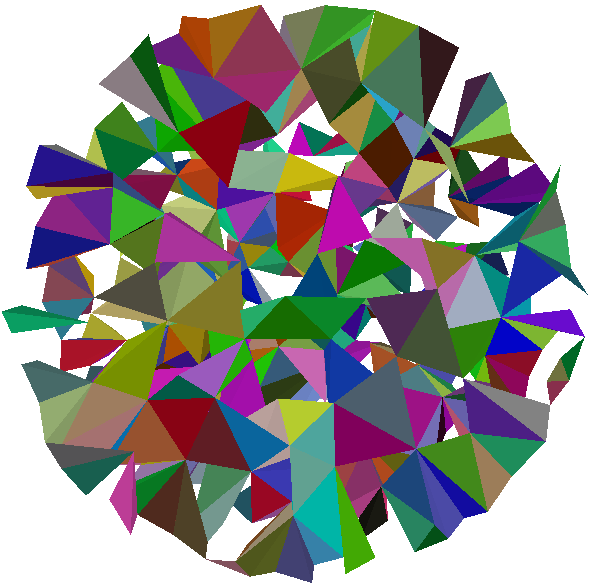
\includegraphics[scale=0.2]{Images/isolated_tetra}
  \caption{figure}{Vue de coupe des tétraèdres isolés après exécution du parcours en largeur pour créer les diamants. Chaque couleur représente un tétraèdre.}
  \label{fig:isolated_tetra}
\end{minipage}%
\begin{minipage}{.5\textwidth}
  \centering
  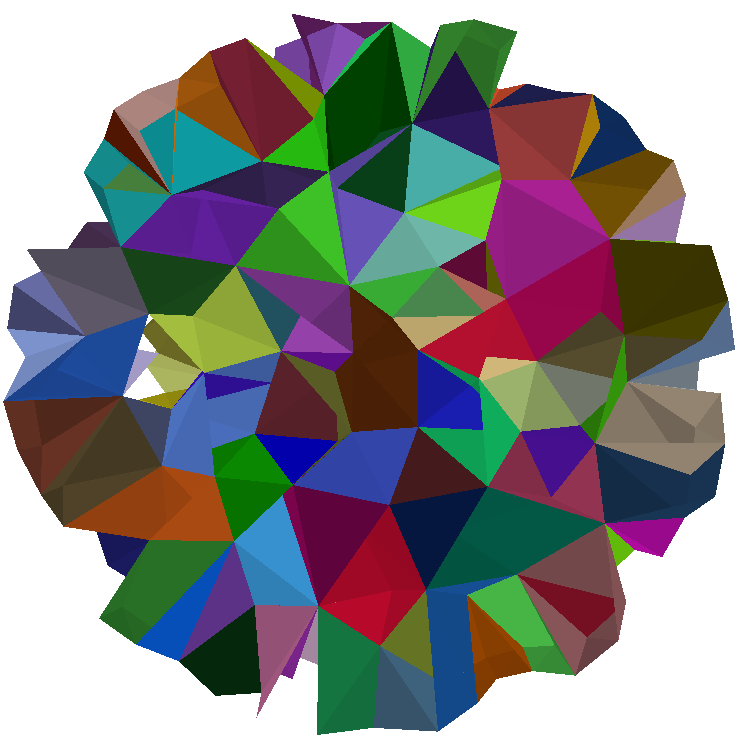
\includegraphics[scale=0.16]{Images/diamond}
  \caption{figure}{Vue de coupe des diamants après exécution du parcours en largeur pour créer les diamants. Chaque couleur représente un diamant.}
  \label{fig:diamond}
\end{minipage}
\end{figure}
\noindent
Sur Fig. \ref{fig:isolated_tetra}, on note une certaine homogénéité des tétraèdres isolés. En analysant plus spécifiquement la concentration des tétraèdres isolés, on remarque sur les Fig. \ref{fig:density_cow} et Fig. \ref{fig:hand_density} qu'ils sont particulièrement situé sur les bords et dans des régions à courbures \footnote{Afin que la densité ne soit pas biaisée, nous avons soustrait la densité originale du maillage. Le fait qu'une région soit plus densément peuplée en tétraèdre n'influence donc pas le résultat.}.
\begin{figure}[H]
\centering
\begin{minipage}{.5\textwidth}
  \centering
  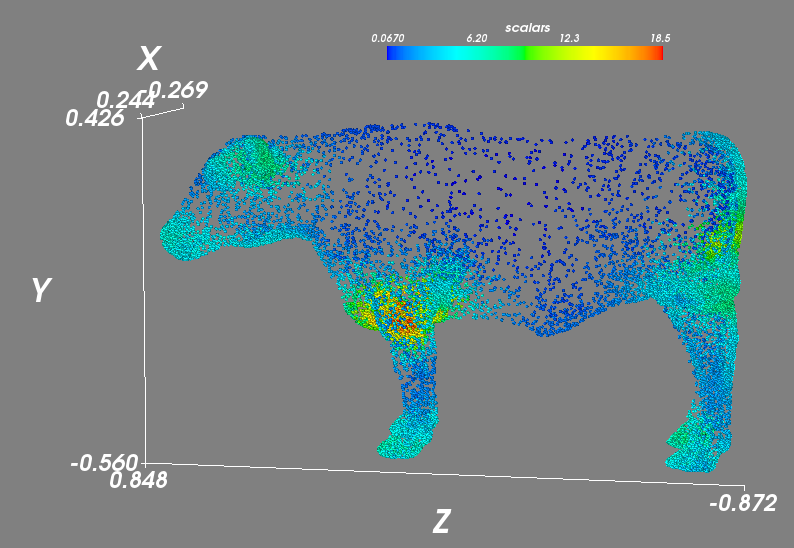
\includegraphics[scale=0.3]{Images/density_cow}
  \caption{figure}{Distribution des tétraèdres isolés. Chaque point représente le barycentre d'un tétraèdre et sa couleur indique la densité (le nombre de tétraèdres isolés à proximité).}
  \label{fig:density_cow}
\end{minipage}%
\begin{minipage}{.5\textwidth}
  \centering
  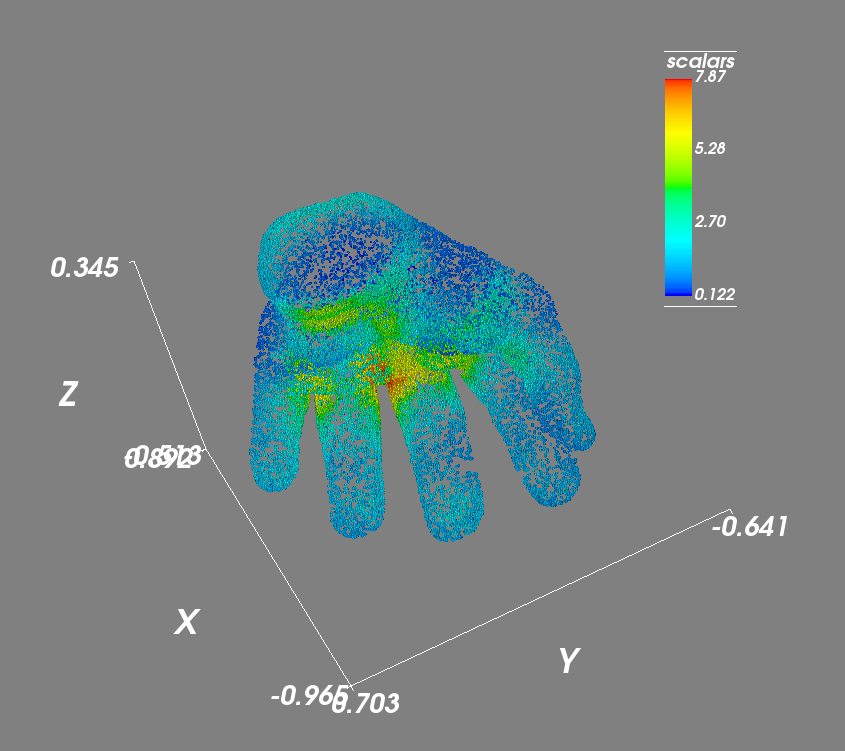
\includegraphics[scale=0.23]{Images/hand_density}
  \caption{figure}{Distribution des tétraèdres isolés. Chaque point représente le barycentre d'un tétraèdre et sa couleur indique la densité (le nombre de tétraèdres isolés à proximité).}
  \label{fig:hand_density}
\end{minipage}
\end{figure}

\paragraph{Choix du tétraèdre de départ}
Suivant le premier tétraèdre choisi pour lancer l'algorithme de parcours en largeur (fig. \ref{fig:bfs_starting}), le taux de tétraèdres appareillés dans des diamants varie peu (1\% d'écart). Il semble néanmoins plus intéressant de commencer par les régions étroites.
\begin{figure}[H]
\begin{center}
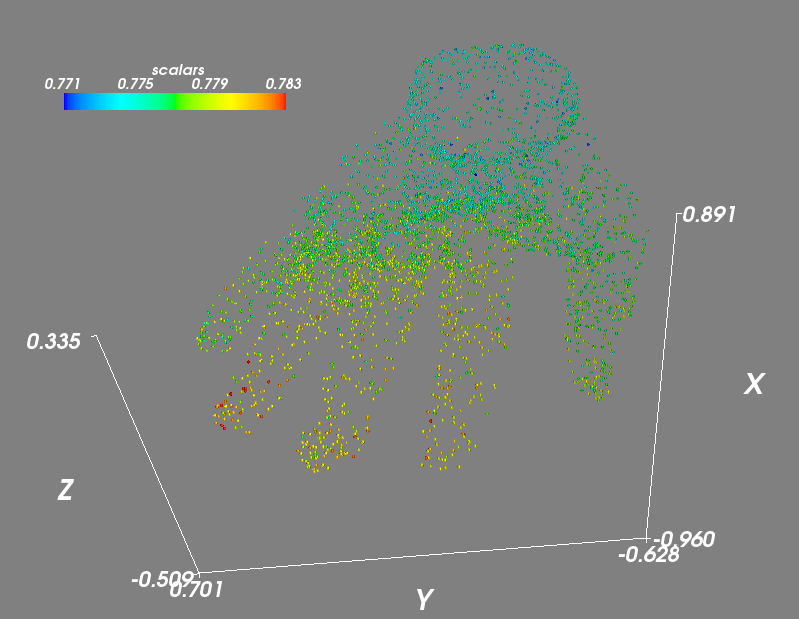
\includegraphics[scale=0.3]{Images/bfs_starting}
\caption{Performance de l'algorithme de parcours en largeur en fonction du tétraèdre de départ.}
\label{fig:bfs_starting}
\end{center}
\end{figure}
\noindent

\paragraph{Avantages et inconvénients}
L'algorithme de parcours en largeur du graphe est très rapide car sa compléxité est linéaire par rapport à la taille du graphe. De plus, son implémentation est très facile et permet à quiconque de le ré-implémenter ou de le modifier. En revanche, environ 20\% des tétraèdres demeurent isolés et ceux-ci sont principalement localisés sur les bords du volume. Parcourir en largeur les tétraèdres est un comportement naïf. Un algorithme ayant une vision globale du maillage et non juste locale aurait probablement de meilleures performances. 
\subsubsection{Optimisation aléatoire}
\noindent
Notre problème s'exprime facilement comme un problème d'optimisation combinatoire en nombres entiers. Malheureusement, la résolution de ces problèmes NP-difficile, ce qui signifie qu'aucun algorithme ne peut trouver une solution optimale en temps polynomial. Néanmoins, on peut utiliser des algorithmes d'optimisation aléatoire afin de trouver une solution approchée. Ce sont des algorithmes très utilisés en pratique qui visitent plus ou moins aléatoirement l'espace des solutions.\\
Soit $f$ la fonction aléatoire à minimiser, l'idée est de partir d'une solution initiale x et tant que la condition d'arrêt n'est pas remplie, de créer une solution y à partir de x puis de remplacer x par y si f(y)$>$f(x).\\
Dans notre cas, une solution est un ensemble d'arêtes. Elle est faisable si pour toute paire d'arêtes de notre solution, aucunes n'appartiennent au même tétraèrdre. On peut donc matérialiser notre solution comme un vecteur de 0 et 1 pour chaque arête du graphe (1 si l'arête appartient à la solution, 0 sinon). Pour calculer la valeur de notre solution, on ajoute pour chaque arête de la solution le nombre de tétraèdre utilisant l'arête et si deux arêtes appartienent au même tétraèdre alors on inflige une pénalité en soustrayant le nombre de tétraèdres adjacents à ces deux arêtes.\\
L'inconvénient majeur de cet algorithme est sa lenteur. En effet, il permet de trouver des solutions quasi optimales pour des maillages à plusieurs milliers d'arêtes en quelques secondes mais ne permet pas de trouver des solutions convenables au dela.\\
Par conséquent, nous avons décidé de joindre l'algorithme de parcours en largeur et l'algorithme randomisé pour allier les avantages des deux : la rapidité de BFS et la globalité d'optimisation aléatoire.
\subsubsection{Parcours en largeur et optimisation aléatoire}
\noindent
La solution finale est donc un mélange de BFS et d'algorithme randomisé. BFS offre une solution convenable en un temps très court. Néanmoins, sa solution peut etre améliorer avec un algorithme randomisé.
Nous avons donc sélectionné un ensemble d'arêtes representant les diamants. Tous les tetrahedres ne possedant pas une de ces aretes sont dit isolés.
\begin{table}[H]
\footnotesize
\begin{tabular}{|c | c | c | c| c | c | c |}
\hline
& \multicolumn{2}{|c|}{BFS}& \multicolumn{2}{|c|}{Algorithme randomisé} & \multicolumn{2}{|c|}{BFS et randomisé}\\
\hline
Nom de la & Part des tétraèdres & RPT& Part des tétraèdres & RPT& Part des tétraèdres & RPT\\
structure&dans des diamants&&dans des diamants&&dans des diamants&\\
\hline
B1 & 0.76 & 2.69\\
B2 &  0.80 & 2.39\\
B3 & 0.81 & 2.37\\ 
V1 & 0.77 & 2.44\\ 
M1 &  0.77 & 2.44\\ 
C1 &  0.77 & 2.44\\ 
\hline  
\end{tabular}
\label{Tab:results_performances}
\end{table}
\begin{figure}[H]
\begin{center}
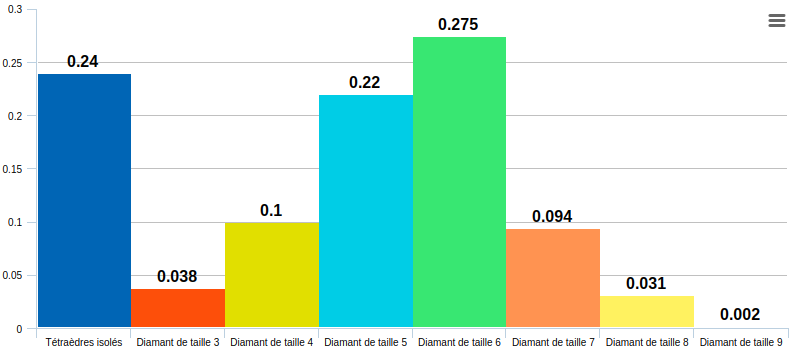
\includegraphics[scale=0.45]{Images/histograme}
\caption{Histograme de la part de tétraèdres parmi les tétraèdres isolés et diamants}
\label{fig:bfs_starting}
\end{center}
\end{figure}


\subsection{Choisir l'ancre}
\noindent
Le but de cette section est d'associer chaque sommet à un diamant ou un tétraèdre isolé. Voici les règles pour l'association.\\
\begin{itemize}
\item Un diamant ne peut être associé qu'à un sommet de son arête centrale
\item Un tétraèdre isolé peut être associé à n'importe lequel de ses quatres sommets
\item On associe en priorité les sommets à des diamants afin de calculer plus rapidement le degré du sommet
\end{itemize}
\begin{figure}[H]
\centering
\begin{minipage}{.5\textwidth}
  \centering
  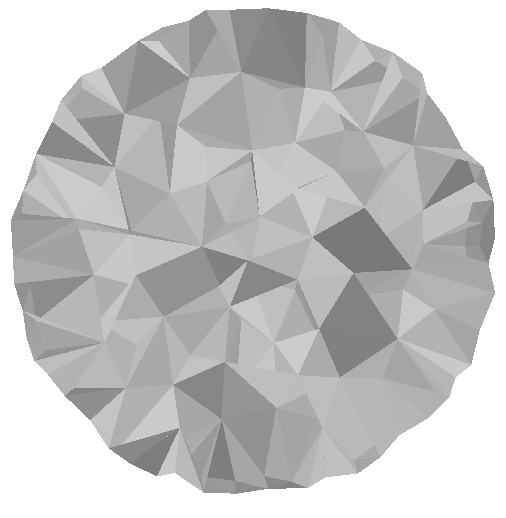
\includegraphics[scale=0.2]{Images/half_ball}
  \caption{figure}{Vue de coupe d'une tétraèdrisation d'une boule}
  \label{fig:half_ball}
\end{minipage}%
\begin{minipage}{.5\textwidth}
  \centering
  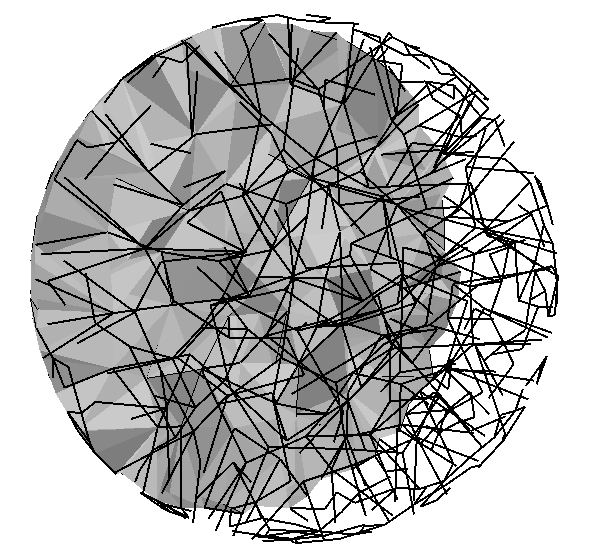
\includegraphics[scale=0.2]{Images/central_edges}
  \caption{figure}{Vue de coupe d'une tétraèdrisation d'une boule avec l'affichage des arêtes centrales de tous les diamants}
  \label{fig:central_edges}
\end{minipage}
\end{figure}
\noindent
Les différents cas possibles pour l'association des sommets sont les suivants :\\
\begin{itemize}
\item Le sommet est adjacent à une arête centrale disponible. On associe le sommet à cette arête.
\item Le sommet n'est adjacent à aucune arête centrale et il est adjacent à un tétraèdre isolé libre. Alors on associe le sommet à ce tétraèdre libre.
\item Le sommet n'est adjacent à aucune arête centrale, n'est pas adjacent à un tétraèdre isolé libre mais est adjacent à un diamant. On "explose" alors le diamant, c'est à dire qu'on fait comme s'il était constitué que de tétraèdres isolés. Sur la Fig. \ref{fig:central_edge_AB}, le sommet F n'est pas sur une arête centrale. Si le diamant est déjà associé au sommet A (resp. B) alors on explose le diamant. On peut alors associer le sommet F (Fig. \ref{fig:explosion_diamond}) aux tétraèdres ABFG ou ABFC et le sommet A (resp. B) aux tétraèdres ACDB ou ADEB ou ABEG.
\end{itemize}

\begin{figure}[H]
\centering
\begin{minipage}{.5\textwidth}
  \centering
  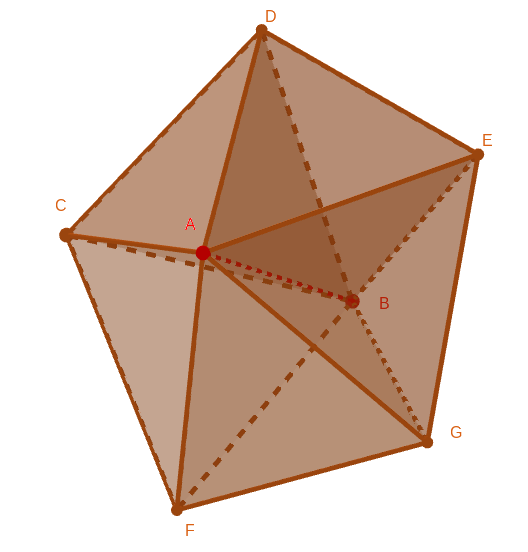
\includegraphics[scale=0.35]{Images/central_edge_AB}
  \caption{figure}{Image d'un diamant contenant 5 tétraèdres dont l'arête centrale est le segment AB et ancré au sommet A}
  \label{fig:central_edge_AB}
\end{minipage}%
\begin{minipage}{.5\textwidth}
  \centering
  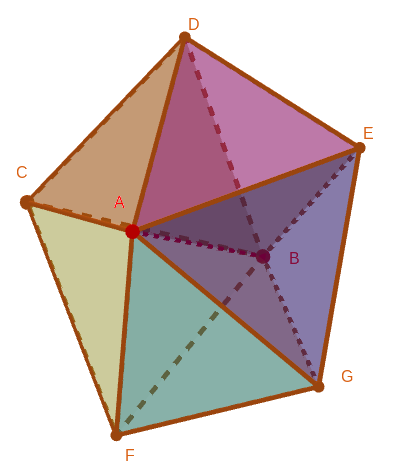
\includegraphics[scale=0.42]{Images/explosion_diamond}
  \caption{figure}{Image de 5 tétraèdres isolés (chaque couleur est un tétraèdre différent)}
  \label{fig:explosion_diamond}
\end{minipage}
\end{figure}
En utilisant un algorithme glouton qui affecte en priorité les sommets adjacents à peu d'arêtes centrales, nous sommes capables d'appareiller \%\% des sommets avec des diamants.
\begin{table}[H]
\footnotesize
\begin{tabular}{|c | c | c | c |}
\hline
Nom de la & Part de sommets non associés & Part de tétraèdres dans  & Part de tétraèdres dans \\
structure&avec des diamants  & des diamants avant & des diamants après \\
& ou tétraèdres isolés & choix des ancres& choix des ancres\\
\hline
B1 & 0.06 & 0.76 & 0.65 \\
B2 & 8e-4 & 0.80 & 0.80 \\
B3 &  & 0.82 & \\
V1 & 8e-3  & 0.77 & 0.76 \\
M1 & 7e-3 & 0.77 & 0.76\\
C1 & 8e-3 & 0.77 & 0.76 \\
\hline  
\end{tabular}
\label{Tab:results_ancres}
\end{table}

\begin{figure}[H]
\begin{center}
%\includegraphics[scale=0.2]{Images/image_arete_couleur_avec_sommet}
%\caption{Exemple de diamant}
%\label{fig:tetra_depart}
\end{center}
\end{figure}
\noindent
On s'aper\c coit que la destruction de certains diamants pour associer des sommets à des tétraèdres n'a que peu d'incidence sur les performances tant que le nombre de sommets est important (tableau \ref{Tab:results_ancres}).

\subsection{La structure}
\noindent
Désormais, nos diamants sont formés et les sommets sont associés à des diamants (ou des tétraèdres isolés).\\
Pour rappel, notre structure doit permettre de :
\begin{itemize}
\item Accéder au ième tétraèdre en temps constant
\item Accéder au ième sommet en temps constant
\item Naviguer facilement dans le graphe (entre les tétraèdres)
\item Calculer le degré (i.e l'hypersphère) d'un sommet
\end{itemize}
La structure que nous proposons est un tableau $F$ à une dimension dont la taille est le nombre de faces extérieures des diamants ou tétraèdres isolés. Les faces extérieures sont toutes les faces des tétraèdres isolés et les faces externes des diamants. Le tableau contient des entiers qui sont les indices des faces. Ainsi F[i] indique l'indice dans le tableau de la face adjacente à la ième face. Si la ième face est sur le bord du volume alors F[i]=-1.\\ 
Un diamant contenant quatre tétraèdres occupera 8 cellules dans le tableau (car il a 8 faces extérieures) et un tétraèdre isolé en occupera 4. Les diamants sont ré-ordonnés de tel manière que le ième sommet soit ancré au ième diamant. Etant donné qu'il y a beaucoup plus de diamants que de sommets, seuls, les $|V|$ premiers diamants sont ré-ordonnés.\\
Par ailleurs, pour savoir quand on passe d'un diamant à un autre, nous utilisons des bits de service (1 ou 0) pour chaque face. Une face contient un 1 si c'est la première face d'un diamant, 0 sinon. Finalement, afin de pouvoir tourner facilement autour d'un sommet, nous utilisons 3 bits de service par face pour représenter la permutation des sommets entre ces deux faces.\\
Pour résumer, voici notre structure de données :
\begin{itemize}
\item Un tableau de tailles |F| où F est l'ensemble des faces exterieures du maillage.
\item Un bit de service par face afin de savoir si une face est la première d'un diamant ou d'un tétraèdre isolé
\item 3 bits de service par face afin de représenter la permutation des sommets entre deux faces
\end{itemize}
\begin{figure}[H]
\begin{center}
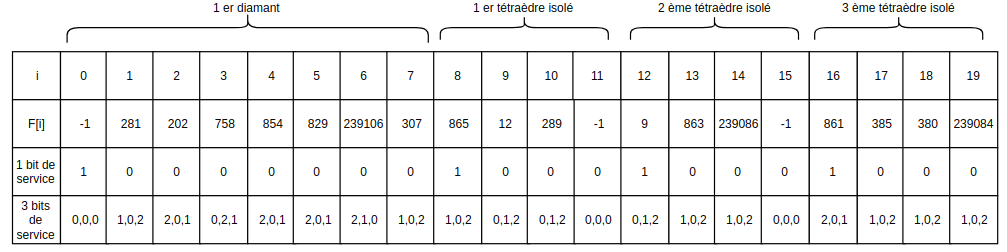
\includegraphics[scale=0.45]{Images/structure}
\caption{Notre structure est constituée d'un tableau F contenant les indices des faces adjacentes, d'un bit de service permettant de savoir si une face est la première d'un diamant ou d'un tétraèdre, et de trois autres bits de service afin de connaître la permutation des sommets entre deux faces. Dans cet exemple, la face 0 est sur le bord et la face 1 est adjacente à la face 281.}
\label{fig:structure}
\end{center}
\end{figure}

\paragraph{Ordre des tétraèdres dans un diamant}
Au sein d'un diamant les tétraèdres sont ordonnés de manière purement arbitraire (Fig. \ref{fig:tetra_ordonnee}). La seule condition est que deux tétraèdres adjacents doivent avoir un ordre consécutif modulo le nombre de tétraèdres dans le diamant (ex: dans un diamant contenant 5 tétraèdres, le troisième tétraèdre doit être adjacent au deuxième tétraèdre et au quatrième).
\paragraph{Ordre des faces dans un diamant}
L'ordre des faces dans un diamant respecte celui des tétraèdres. Pour le ième tétraèdre dans un diamant, ses faces extérieures seront les faces $2i$ et $2i+1$. Si un diamant est associé à un sommet alors les faces paires sont adjacentes à l'ancre. Sur la Fig. \ref{fig:tetra_ordonnee}, l'ordre des face est donc : ACD,BCD,ADE,BDE,AGE,BGE,AFG,BFG,AFC,BFC.
\paragraph{Ordre des faces dans un tétraèdre isolé}
Les faces d'un tétraèdre isolé sont ordonnées de manière arbitraire. Seulement, si le tétraèdre isolé est associé à un sommet, alors la première face doit être la face opposée à l'ancre.
\paragraph{Ordre des sommets dans les diamants}
\label{Ordre des sommets dans les diamants}Tout comme les tétraèdres, les sommets peuvent être ordonnés au sein d'un diamant. Un diamant D possedant $|D|$ tétraèdres contient $|D|+2$ sommets. On ordonne d'abord les sommets situés entre deux faces (les sommets D,E,G,F,C sur la Fig. \ref{fig:tetra_ordonnee}), puis les deux sommets communs à toutes les faces (les sommets A et B sur la Fig. \ref{fig:tetra_ordonnee}). Le classement entre ces deux-derniers n'est pas important car on ne compare jamais l'ordre de ces deux sommets.
\begin{figure}[H]
\begin{center}
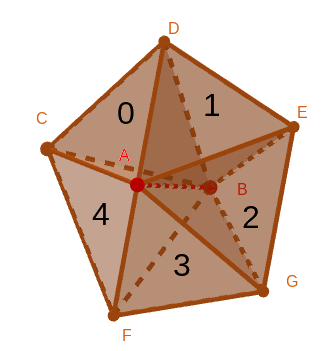
\includegraphics[scale=0.45]{Images/tetra_ordonnee}
\caption{Diamant contenant 5 tétraèdres ordonnés, dont l'arête centrale est AB et ancré au sommet A. L'ordre des tétraèdres est indiqué en noir. L'ordre des sommets est : C,D,E,G,F,A,B.}
\label{fig:tetra_ordonnee}
\end{center}
\end{figure}
\noindent
\paragraph{Ordre des sommets dans les tétraèdres}
Au sein d'un tétraèdre, les sommets sont ordonnés tel-que le ième sommet est opposé à la ième face. Si un sommet est associé au tétraèdre alors ce sommet est opposé à la première face.
\subsection{Calculer les permutations}
\noindent
\begin{figure}[H]
\begin{center}
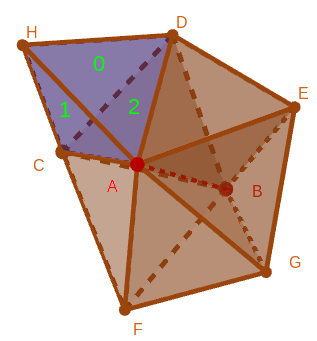
\includegraphics[scale=0.45]{Images/permutation_tetra_diamant}
\caption{Un diamant partage une face avec un tétraèdre isolé. En vert est l'ordre des face du tétraèdre. L'ordre des sommets du tétraèdre est A,D,C,H et celui du diamant est C,D,E,G,F,A,B.}
\label{fig:permutation_tetra_diamant}
\end{center}
\end{figure}
\noindent
Pour calculer la permutation vue du tétraèdre isolé de la face CAD, il suffit de comparer l'ordre des sommets du tétraèdre isolé et du diamant. Si l'on garde seulement les 3 sommets qui nous intéresse dans les deux classements, on a : A,D,C et C,D,A. La permutation est donc (2,1,0). Bien entendu, la permutation pour la même face du point de vue du diamant est la même.\\
Il y a 3!=6 permutations possibles et donc 3 bits sont nécessaires pour représenter ces permutations.
\subsection{Les requêtes}
\subsubsection{Vérifier qu'un diamant est correct}
\noindent
Cette fonction est essentielle car elle nous permet de savoir si une arête peut être candidate pour être l'arête centrale d'un diamant. Pour cela, on vérifie que deux sommets apparaissent plus de deux fois, et tous les autres apparaissent exactement deux fois.
\begin{lstlisting}
bool is_cycle(vector<Tetrahedron*>& tetra_list)
{
    map<int,int> count_vertex;
    for (int i=0;i<tetra_list.size();i++)
    {
        for (Vertex* j : tetra_list[i]->get_vertices())
        {
            count_vertex[j->get_id()]+=1;
        }
    }
    for (pair<int,int> i : count_vertex)
    {
        if (i.second<2)
        {
            return false;
        }
    }
    return true;
}
\end{lstlisting}
\subsubsection{Accéder à la ième face}
\noindent
Pour accéder à la ième face, il suffit d'accéder à la cellule F[i] dans laquelle se trouve la face opposée à la ième face.
\subsubsection{Acceder au ième diamant ou tétraèdre isolé}
\noindent
Il suffit de parcourir le tableau $F$ et de regarder pour chaque face si le premier bit de service vaut 1. On s'arrête alors dès que l'on a parcouru i faces dont la valeur du premier bit de service est 1. La compléxité est O(n).\\
\begin{lstlisting}
int ith_tetra_diamond(bool service_bit_array[],int array_size,int i)
{
    int count=0;
    int j=0;
    while(count<i)
    {
    	if (service_bit_array[j]==1)
    	{
    		count++;
    	}
    }
    return j;
}
\end{lstlisting}
\subsubsection{Parcourir les tétraèdres d'un diamant}
\noindent
Les faces au sein d'un diamant sont ordonnées. Les faces consécutives dans le tableau (modulo la taille du diamant) sont adjacentes dans le diamant. Par conséquent, pour aux face du ième tétraèdre d'un diamant D, il suffit d'aller à la $2i$ et $2i+1$ ième face du diamant (modulo $|D|$).
La compléxité est O(1).
\subsubsection{Acceder au ième tétraèdre}
\noindent
Lors du regroupement des tétraèdres en diamants, l'ordre des diamants n'est plus le même que l'ordre initial (à la lecture du fichier OFF). Néanmoins, on peut re-ordonner les tétraèdres dans le fichier original afin que l'ordre des tétraèdres soit les mêmes. De cette manière on peut acceder au ième tetra en O(n).
\subsubsection{Acceder au ième sommet}
\noindent
Bien que nous ne stockions pas les sommets de manière explicites (nous ne stockons que les faces). Nous sommes en mesures de localiser le ième sommet car il est adjacent au ième diamant/tétraèdre isolé.
Il suffit donc d'accéder au ième diamant/tétraèdre isolé. Si c'est un diamant, alors le sommet est adjacent à toutes les faces paires du diamant. Si c'est un tétraèdre isolé, alors le sommet est opposé à la première face et est donc adjacent au trois autres faces. La compléxité est O(n).
\subsubsection{Degré et hypersphère d'un sommet}
\noindent
Calculer le degré d'un sommet est plus compliqué. On sait que le ième sommet est adjacent au ième diamant/tétraèdre isolé. Si celui-ci est un diamant alors toutes les faces paires de celui-ci sont adjacentes au sommet ciblé. Si c'est un tétraèdre isolé, alors le sommet cible est opposé à la première face et est donc adjacent aux trois autres faces. Pour chaque face adjacente au sommet on accède à la face opposée en utilisant notre tableau $F$. En utilisant les permutations entre deux faces, nous sommes en mesure de savoir où se situe notre sommet dans la face opposée. Ainsi, nous pouvons accéder aux faces adjacentes au sommet dans ce nouveau diamant/tétraèdre isolé. Pour chaque diamant/tétraèdre isolé, on utilise un bit de service afin de savoir si celui-ci a déjà été visité \footnote{Nous omettons ce bit de service car il y en a en moyenne $\frac{|Diamants| + |T\acute{e}tra\grave{a}dres \; isol\acute{e}s|}{|T\acute{e}tra\grave{a}dres|}\simeq 0.5$ par tétraèdre}.. On arrête de parcourir les faces quand tous les diamants et tétraèdres isolés adjacents au sommet ont été visités.
\subsubsection{Parcours en profondeur du graphe}
\noindent
Parcourir en profondeur le graphe est plus facile que de calculer le degré d'un sommet. Il suffit d'utiliser une file et un bit de service pour chaque tétraèdre afin de savoir si celui-ci a été visité. Le passage d'un tétraèdre à l'autre est rendu très facile grace à notre tableau représentant les faces adjacentes.
\begin{lstlisting}
void BFS(int diamond_array[],bool service_bit_array[],int array_size,
int starting_index)
{
    queue<int> wait_list;
    unordered_set<int> visited_polygons; 
    int index = ith_diamond(service_bit_array,array_size,starting_index);    
    wait_list.push(get_starting_index(service_bit_array,index)); 
    while(!wait_list.empty())
    {
        index = wait_list.front();
        wait_list.pop();
        int i=index+1;
        int diamond_id = get_starting_index(service_bit_array,index);
        if(visited_polygons.count(diamond_id)==0)
        {
            visited_polygons.insert(diamond_id);
            path.push_back(diamond_id);
            //we iterate over the following faces in the diamond or isolated tetra
            while(service_bit_array[i]!=1 && i<array_size)
            {
                if (diamond_array[i]!=-1)
                {
                    wait_list.push(diamond_array[i]);
                }
                i++;               
            }
            //we iterate over the previous faces in the diamond or isolated tetra
            i=index;
            while(service_bit_array[i]!=1 && i<array_size)
            {
                if (diamond_array[i]!=-1)
                {
                    wait_list.push(diamond_array[i]);
                }
                i--;
            }
            if (diamond_array[i]!=-1)
            {
                wait_list.push(diamond_array[i]);
            }
        }
    }
}

\end{lstlisting}

\subsubsection{Retrouver l'indice d'un sommet}
\label{Retrouver l'indice d'un sommet}
\noindent
Retrouver l'indice d'un sommet est une procédure courante. En effet lorsque on est sur une face, on peut vouloir connaître les trois sommets qui la compose. Pour connaître l'indice d'un sommet, on calcule son hypersphère. Puis pour chaque diamant ou tétraèdre isolé dans l'hypersphère dont l'indice de la première face est inférieur à la limite\footnote{La limite est l'index à partir duquel les diamant et tétraèdres isolés ne sont plus associés à des sommets}, on calcule alors l'hypersphère du sommet ancré. Il suffit alors de comparer l'hypersphère de notre sommet cible avec les hypersphère des sommets ancrés et de renvoyer l'indice du sommet ayant la même hypersphère. Cette opération peut s'avérer néanmoins très couteuse. La compléxité pour calculer l'hypersphère d'un sommet est O(d). En moyenne, en utilisant notre algorithme pour appareiller les tétraèdres en diamants, les sommets sont en moyennes adjacents à 8 diamants/tétraèdres isolés. Seulement parmi, ces 8 diamants/tétraèdres isolés, en moyenne 65\% auront un indice inférieur à la limite. Par conséquent, retrouver l'indice d'un sommet nécessite de calculer en moyenne 6 (0.65*8+1) hypersphères.
\subsection{Resultats}
\noindent
\begin{table}[H]
\footnotesize
\begin{tabular}{|c | c | c | c | c| c |c |}
\hline
Nom de la & Construire les & Choisir les arêtes centrales & Accès au& Accès au & Degré d'un & Parcours en\\
structure & diamants & et appareiller sommet/diamant &ième tétraèdre& ième diamant &sommet&prodondeur\\
\hline
B1 & 0.02 & 0.06 & 1e-5 & 5e-6 & 1.9e-5 & 6e-4\\
B2 & 0.86 & 12.94 &  4.1e-4 & 1.6e-4 & 1.2e-4 & \\
%Boule & 33.29
%Vache & 1.37 & 
M1 & 1.09 & 50.6 & 6.4e-4 & 2.6e-4 & 2.2e-4 & \\
C1 & 1.42 & 96.71 & 8.1e-4 & 3.4e-4 & 2.8e-4 & \\
\hline  
\end{tabular}
\label{Tab:results_time}
\end{table}
\noindent
Les résultats du tableau \ref{Tab:results_time} sont obtenus en utilisant l'optimisation "-O3" de C++. Les résultats obtenus sont des moyennes calculées après 10 000 essais.

\begin{table}[H]
\footnotesize
\begin{tabular}{|c | c | c |}
\hline
Type de & Taille du & Mémoire consomée \\
structure & tableau de diamant & totale \\
\hline
Boule & & \\
Boule & & \\
Boule & & \\
Vache &  & \\
Main &  & \\
Tête &  & \\
\hline  
\end{tabular}
\label{Tab:results_memory}
\end{table}
\noindent


\subsection{Borne inférieure théorique}

\subsection{Sauvegarder notre structure}
\noindent
Les fichiers OFF encodent d'abord les coordonnées géométriques de chaque sommet puis les indices des 3 sommets de chaque face. Ils sont ainsi très faciles à manipuler mais ne sont pas concis (un sommet apparaît en moyenne 18 fois dans une tétraèdrisation AJOUTER FOOTNOTE).
\paragraph{Encodage de la structure}
Comme dit dans la partie \ref{Retrouver l'indice d'un sommet}, un sommet dans notre structure est adjacent en moyenne à 8 diamants/tétraèdres isolés. Par conséquent, plutôt que de décrire pour chaque face les 3 indices des 3 sommets, nous pouvons encoder les indices des sommets composant un diamant. Comme nous l'avons vu dans la partie \ref{Ordre des sommets dans les diamants}, les sommets sont ordonnés dans un diamant. Par conséquent, en ayant juste l'ordre des sommets, nous sommes en mesure de retrouver les faces (la première face est bordée par le premier, le deuxième et l'avant dernier sommet).\\
Cependant, notre structure ne stocke pas implicitement les sommets. Nous savons seulement que le ième sommet est adjacent au ième diamant/tétraèdre isolé. Néanmoins, en calculant l'hypersphère de d'un sommet, nous informons les faces adjacentes qu'elles possèdent ce sommet. En faisant ainsi pour tous les sommets du maillage, nous associons alors à chaque face ses 3 sommets bordants.\\
Il est alors facile de retrouver l'ordre des sommets dans un diamant à partir des sommets bordants chaque face du diamant. Il suffit de prendre tous les sommets qui apparaissent exactement deux fois dans toutes les faces (i.e les sommets qui n'appartiennent pas à l'arête centrale). Puis de les ordonner afin qu'ils décrivent un cycle.\\
Par exemple, sur la Fig. \ref{fig:tetra_ordonnee}, à partir du calcul de l'hypersphère de chaque sommet, nous saurions alors que :
\begin{itemize}
\item Les faces 0 et 1 contiennent les sommets C et D
\item Les faces 2 et 3 contiennent les sommets E et D
\item Les faces 4 et 5 contiennent les sommets G et E
\item Les faces 6 et 7 contiennent les sommets F et G
\item Les faces 8 et 9 contiennent les sommets C et F
\end{itemize}
Trouver l'ordre des sommets est alors aisé. On commence par trouver le sommet commun à la première et dernière face (i.e C), puis le sommet commun à la première et deuxième face (i.e D) et ainsi de suite pour finalement obtenir : C,D,E,G,F,A,B (les deux derniers sommets sont communs à toute les faces).\\

\paragraph{Ecriture dans un fichier}
L'écriture dans un fichier suit le même procédé que pour les fichiers OFF. Nous écrivons d'abord les coordonées géométriques de chaque sommet. Puis nous écrivons pour chaque diamant et tétraèdre isolé l'ordre de ses sommmets.

\paragraph{Ouverture du fichier}
L'ouverture est similaire à l'encodage du maillage. Pour chaque diamant, l'ordre des sommets nous permet de connaître les faces. Pour chaque tétraèdre isolé, l'ordre n'est pas important étant donné que tous les sommets d'un tétraèdre sont adjacents.

\paragraph{Résultats}
En théorie comme en pratique, notre structure nous permet d'économiser en moyenne 44\% ($\frac{8}{18}$) de références dans le fichier OFF.

\subsection{Améliorations}
\subsubsection{Références différentielles}
\noindent
Dans notre tableau T, chaque face est représenté par un indice sur 32 bits, qui est la taille miimale d'un entier en C++. Néanmoins, on peut representer l'adjacence par la sa distance entre les deux faces dans le tableau.\\
Malheureusement, les faces sont seulement ordonneés de manière à ce que le sommet soit adjacent au ième diamant. Par conséquent, nous n'avons aucune garanti sur l'éloignement (dans le tableau $F$) de deux faces opposées. Etant donné que le gain semblait mineur, nous avons choisi de ne pas implémenter cette fonction.

\subsubsection{Dynamicité}
\noindent
Une structure de données compacte est dîtes dynamique lorsqu'on peut modifier les données localement (i.e de manière instantanée). Dans notre cas, modifier les données peut revenir à ajouter un sommet, ajouter une face, supprimer un tétraèdre...\\
Malheureusement, nous n'avons encore implémenté encore aucune de ces fonctions.

\section{NP completude}
Le problème : Existe-il une couverture des tetras en diamants contenant plus de k tetras ?

Apparier les tetras en diamants est l'étape clé de notre algorithme. Malheureuseument, nous montrons dans cette section que ce problème est NP-Complet.
En effet, notre problème consiste à choisir un ensemble d'aretes tel qu'aucune de ces arêtes n'appartiennent au même tetra.
On peut alors créer un autre graphe où chaque arête du graphe initial est modélisé par un sommet. Deux sommets dans ce nouveau graphe sont connectés si et seulement si leur arete dans le graphe original appartiennent au même tetra.
La création de ce nouveau graphe se fait en temps polynomiale (en fonction des arêtes).

Dans ce nouveau graphe, notre problème devient le même que le maximum independant set (MIS). A savoir que l'on recherche un ensemble maximum de sommets (donc d'aretes dans notre graphe initial) tel qu'aucun de ces sommets de soient connectés (donc que leur aretes appartiennent au même tetra dans le graphe initial).
En revanche, notre instance du MIS est une instance pondérée, où chaque sommet à un poids correspondant au nombre de tetra adjacent à l'arete dans le graphe initial.

\section{Implémentation}
\noindent
Tout est implémenté en C\texttt{++} natif, sans l'aide d'aucune bibliothèque extérieure. Tous les algorithmes ont été exécutés sur une machine avec un processeur i5-5300U et 16Go de RAM. L'ensemble du code est open-source et disponible sur github : \url{https://github.com/beaupletga/3D-Mesh-Compression}.\\
Des classes représentent chaque forme géométrique (sommet, tétraèdre, diamant) permettant un code modulable et facilement exploitable. Nous utilisons cette représentation sous forme de classe pour la construction de notre structure mais elle est tout à fait absente dans son utilisation. \\
En ce qui concerne cette dernière, le tableau $F$ est un tableau d'entiers codés sur 32 bits. Bien que nous aurions pu inclure les 4 bits de services dans les 32 bits de chaque entier, nous avons préféré utiliser deux tableaux annexes pour représenter ces bits de service. Le premier bit de service est stocké dans un tableau de booléens et les 3 autres bits de service sont stockés dans un tableau d'entiers. En codant les indices dans le tableau $F$ sur 28 bits et en utilisant les 4 derniers bits comme bits de service, nous pouvons encoder des maillages ayant jusqu'à $2^{28}=268$ millions de faces.

\section{Conclusion}
Afin d'appareiller les tétraèdres en diamants, nous réalisons un parcours en largeur de notre maillage (\ref{parcours_largeur}). Seulement, pour parcourir le maillage, nous lisons entièrement le fichier original car nous n'avons aucune garantie de proximité géométrique dans la manière dont sont énumérés les tétraèdres. C'est le défault principal qui constitue un vrai goulot d'étranglement.

\begin{thebibliography}{999}
\bibitem{triangle_strips}Deering,\emph{Geometry Compression}. 
\bibitem{cut_border_machine_2d}Stefan Gumhold,\emph{Improved Cut-Border Machine for Triangle Mesh Compression}. 
\bibitem{cut_border_machine_3d}Stefan Gumhold, Stefan Guthe, Wolfgang Straßer,\emph{Tetrahedral Mesh Compression with the Cut-Border Machine}. 
\bibitem{edgebreaker}Jarek Rossignac,\emph{Edgebreaker: Connectivity compression for triangle meshes}. 
\bibitem{topological_surgery}Gabriel Taubin, Jarek Rossignac,\emph{Geometric Compression Through Topological Surgery}. 
\bibitem{valence_encoding}Costa Touma and Craig Gotsman,\emph{Triangle Mesh Compression}. 
\bibitem{grow_and_fold}Andrzej Szymczak, Jarek Rossignac,\emph{Grow\&fold: compression of tetrahedral meshes}. 
\bibitem{triangle_strips_weiler}Manfred Weiler, Paula N. Mallon, Martin Kraus, Thomas Ertl,\emph{Texture-Encoded Tetrahedral Strips}. 
\bibitem{SOT}Topraj Gurung, Jarek Rossignac,\emph{SOT: Compact representation for tetrahedral meshes}. 
\bibitem{CGAL},\emph{The CGAL Project. CGAL User and Reference Manual. CGAL Editorial Board, 4.14 edition, 2019}




\end{thebibliography}


\end{document}